\documentclass{iopart}
%\documentclass{article}

\usepackage{hyperref}
\usepackage{color}
\usepackage{graphicx}
\usepackage{harvard}
\usepackage{ulem}
%\usepackage{natbib}

\newcommand{\vtheta}{\vec{\theta}}
\newcommand{\Nbox}{N_\mathrm{box}}
\newcommand{\Vbox}{V_\mathrm{box}}

\newcommand{\be}{\begin{equation}}
\newcommand{\ee}{\end{equation}}
\newcommand{\bel}[1]{\begin{equation}\label{#1}}
\newcommand{\ba}{\begin{eqnarray}}
\newcommand{\ea}{\end{eqnarray}}
\newcommand{\bal}[1]{\begin{eqnarray}\label{#1}}

\newcommand{\ilya}[1]{{\color{red} \bf #1}}
\newcommand{\will}[1]{{\color{blue} \bf Will: #1}}

\newcommand{\order}[1]{\mathcal{O}\left( #1 \right)}

\def\aj{Astron. J.}                 % Astronomical Journal
\def\apj{Astrophys. J.}                % Astrophysical Journal
\def\apjl{Astrophys. J. Lett.}             % Astrophysical Journal, Letters
\def\pasj{PASJ}
\def\apjs{Astrophys. J., Suppl. Ser.}              % Astrophysical Journal, Supplement
\def\mnras{Mon. Not. R. Astron. Soc.}            % Monthly Notices of the RAS
\def\prd{Phys. Rev. D}       % Physical Review D
\def\prl{Phys. Rev. Lett.}    % Physical Review Letters
\def\cqg{Class. Quant. Grav.}%Classical and Quantum Gravity
\def\araa{Annu. Rev. Astron. Astrophys.}             % Annual Review of Astron and Astrophys
\def\nat{Nature}              % Nature
\def\aap{Astron. Astrophys.}                % Astronomy and
                                % Astrophysics
\def\jasa{J. Am. Stat. Assoc.}
\def\pccp{Phys. Chem. Chem. Phys.}
\def\jrssb{J. R. Stat. Soc. B}
\def\aipcs{AIP Conf. Ser.}
\def\jcp{J. Chem. Phys.}

\bibliographystyle{jphysicsB}

\begin{document}
\title[Efficient Jump Proposals in RJMCMC]{An Efficient Interpolation
  Technique for Jump Proposals in Reversible-Jump Markov Chain Monte
  Carlo Calculations}

\date{\today}

\author{W M Farr$^{1,3}$, I Mandel$^{2,3}$ and D Stevens$^{1,4}$}

\address{$^1$ Center for Interdisciplinary Exploration and Research in
  Astrophysics (CIERA), Department of Physics and Astronomy,
  Northwestern University, Evanston IL USA}

\address{$^2$ MIT Kavli Institute, Cambridge MA USA}

\address{$^3$ School of Physics and Astronomy, University of
  Birmingham, Birmingham UK}

\address{$^4$ Department of Astronomy, The Ohio State
  University, Columbus OH USA}


\eads{\mailto{w.farr@bham.ac.uk}, \mailto{imandel@star.sr.bham.ac.uk} \mailto{dan.stevens@u.northwestern.edu}}

\begin{abstract}
  Selection among alternative theoretical models given an observed
  data set is an important challenge in many areas of physics and
  astronomy.  Reversible-jump Markov chain Monte Carlo (RJMCMC) is an
  extremely powerful technique for performing Bayesian model
  selection, but it suffers from a fundamental difficulty: it requires
  jumps between model parameter spaces, but cannot retain a memory of
  the favored locations in more than one parameter space at a time. \ilya{[Not quite true -- see 2.3 -- maybe we can find a better way of saying this in the abstract that doesn't require caveats?]}
  Thus, a naive jump between parameter spaces is unlikely to be
  accepted in the MCMC algorithm and convergence is correspondingly
  slow.  Here we demonstrate an interpolation technique that uses
  samples from single-model MCMCs to propose inter-model jumps from an
  approximation to the single-model posterior of the target parameter
  space.  The interpolation technique, based on a kD-tree data
  structure, is adaptive and efficient in modest dimensionality.  We
  show that our technique leads to dramatically improved convergence
  over naive jumps in an RJMCMC, and compare it to other proposals in
  the literature to improve the convergence of RJMCMCs.  We also
  demonstrate the use of the same interpolation technique as a way to
  construct efficient ``global'' proposal distributions for
  single-model MCMCs without prior knowledge of the structure of the
  posterior distribution, and discuss improvements that permit the
  method to be used in higher-dimensional spaces efficiently.
\end{abstract}

\pacs{02.70.Tt, 95.75.Pq, 07.05.Kf}

\submitto{\CQG}

\maketitle

\section{Introduction}

Selection among alternative theoretical models given an observed data
set is an important challenge in many areas of physics and astronomy.
In a Bayesian context, model selection involves computing the evidence
for \sout{each model given the data} \ilya{the data given each model}.  The model evidence is an integral of
the unnormalized posterior probability distribution over the model
parameter space, representing the probability of obtaining the data
set within that model.  Models with larger evidence are preferred; the
ratio of the evidences of two models is the Bayes factor between them.
The product of the Bayes factor and the ratio of prior probabilities
for the two models yields the odds ratio for the models.

There are many ways to compute model evidences.  In low-dimensional
parameter spaces, the unnormalized posterior probability can be
evaluated on a grid or lattice and the integral can be performed
directly.  For many problems or models of interest, however, the
dimensionality of the parameter space is too large to make this approach
practical, and stochastic sampling must be used.  

Markov chain Monte Carlo (MCMC) methods attempt to stochastically
produce parameter samples with density proportional to the posterior
probability distribution.  In MCMC techniques, the primary target is
an accurate estimate of the posterior distribution.  (We note that an
alternative stochastic method for exploring a model parameter space,
nested sampling \cite{Skilling:2004,Skilling:2006,Feroz:2009},
focuses on evidence computation rather than sampling the posterior
probability density functions.)  It is not straightforward to compute
the model evidence from MCMC samples.  The most direct way to estimate
the evidence for a model from MCMC samples is to compute the
harmonic-mean estimator, but this estimator of the evidence suffers
from infinite variance
\cite{NewtonRaftery:1994,Chib:1995,vanHaasteren:2009}.  MCMC
implementations with parallel tempering \cite{EarlDeem:2005} allow
for evidence computation via thermodynamic integration, but these can
be computationally costly.

\cite{Weinberg2009} \ilya{[Not ideal reference style, but without citet, I have no idea how to fix this ;) ]}
gives a method for directly computing
the evidence integral from existing MCMC samples by using a kD-tree
data structure to decompose a parameter space into boxes containing
the MCMC sample points.  The integral is approximated as a sum over
box volumes.  This method is promising, but it is not clear in general
what statistical and systematic errors it introduces and how these are
affected by the shape of the posterior distribution which the
MCMC samples.

When the goal is model selection between several known models, only
the \emph{relative} evidence of each model is needed.  In this
circumstance, the Reversible Jump MCMC technique first introduced in
\cite{Green1995} is one of the most reliable and accurate ways to
compare the models.  Reversible Jump MCMC (RJMCMC), described more
fully in Section \ref{sec:reversible-jump}, performs a standard MCMC
in a superspace that is a direct sum of all the model parameter
spaces.  Such an MCMC involves both intra- and inter-model jumps; the
number of MCMC samples in each model's parameter space is proportional
to that model's relative evidence in the suite of models being
compared.

Implemented naively, RJMCMC has a significant drawback: because the
chain of samples must be Markovian, only the current sample is
available to the algorithm as it is choosing the next sample.  Each
time an RJMCMC transitions between models, the information about the
choices of parameter values in the previous model is lost; subsequent
jumps into that model must ``start fresh,'' and are correspondingly
unlikely to be accepted, delaying convergence of the RJMCMC sample
chain \ilya{(see \Sref{RJMCMC} for a caveat)}.  \cite{Littenberg2009} addressed this issue by proposing a new
method for producing inter-model jumps in an RJMCMC that relies on
interpolating single-model posterior distributions using a box
decomposition of parameter space.

Here we introduce an alternative technique for improving the
acceptance ratio of inter-model jumps in an RJMCMC, leading to
dramatically improved convergence of RJMCMC sample chains.  The
technique uses a kD-tree data structure to construct an approximation
to each model's posterior parameter distribution.  We draw jump
proposals into the model from this approximation to its posterior.
Because jumps are proposed preferentially to locations favored by the
single-model posterior, the RJMCMC compares ``good'' locations in
parameter space across all the models, and convergence is generally
rapid.  We have successfully applied this RJMCMC technique to a 10-way
model selection among alternative mass distribution models for
black-hole X-ray binaries \cite{Farr2010}.  We also provide an example
using this method as an ``asymptotically Markovian''
\cite{terBraak2008} jump proposal in the context of a single-model,
nine-dimensional MCMC in Section \ref{sec:higherdim}.

The method of \cite{Littenberg2009} for producing inter-model jumps in
an RJMCMC relies on a box decomposition of parameter space, using
fixed-sized boxes.  The method cannot adapt to the local structure of
the posterior, and becomes asymptotically inefficient for
high-dimensional parameter spaces or highly peaked posteriors.
Meanwhile, the approximation to the posterior distribution produced by
the kD-tree is a constant-in-box interpolation of the posterior,
similar in spirit to the phase-space density interpolants produced
from N-body positions and momenta in \cite{Ascasibar2005}.  The
kD-tree interpolation is effective in parameter spaces of modest
dimensionality, and is quite space-efficient, requiring $\order{N}$
storage space and $\order{\log N}$ time to produce each proposed jump,
where $N$ is the number of single-model MCMC samples used to construct
the interpolation.

The structure of this paper is as follows.  In Section
\ref{sec:reversible-jump} we introduce in more detail the concept of a
Reversible Jump MCMC, and describe the fundamental difficulty with a
naive jump proposal in an RJMCMC.  In Section \ref{sec:kDTree} we
introduce the kD-tree data structure used to decompose the parameter
space into boxes for interpolation.  In Section \ref{sec:efficiency}
we demonstrate the efficiency gains that are achieved from use of the
interpolated jump proposal.  In Section \ref{sec:higherdim} we give
examples of some other uses of the interpolated jump proposal that
suggest its utility in the context of a single-model MCMC.  Finally,
in Section \ref{sec:conclusion} we offer a summary and some concluding
remarks on the method.

\section{Reversible Jump MCMC}
\label{sec:reversible-jump}

Reversible jump Markov chain Monte Carlo (RJMCMC) \cite{Green1995} is
a technique for Bayesian model comparison.  Below, we give a very
brief introduction to Bayesian analysis, describe a standard MCMC, and
introduce RJMCMC.

\subsection{Bayesian analysis}

Consider an observed data set $d$ and a set of competing models for
the data, indexed by an integer $i$: $\{M_i | i = 1, 2, \ldots \}$.
Each model has some continuous parameters, $\vtheta_i$; given the
model and its parameters, we can make a prediction about the
likelihood of observing the experimental data: $L(d|\vtheta_i, M_i)$.
Within the framework of each model, Bayes' rule gives us a way to
compute the posterior probability distribution function (PDF) for the
model parameters implied by the data:
\be
  p(\vtheta_i | d, M_i) = \frac{L(d|\vtheta_i, M_i) p(\vtheta_i|M_i)}{p(d|M_i)},
\ee
where $p(\vtheta_i |d, M_i)$ is the posterior distribution for the
model parameters $\vtheta_i$ implied by the data in the context of
model $M_i$, $p(\vtheta_i|M_i)$ is the prior probability of the model
parameters that represents our beliefs before accumulating any of the
data $d$, and $p(d|M_i)$, called the evidence, is an overall
normalizing constant that ensures that $p(\vtheta_i|d,M_i)$ is
properly normalized as a probability distribution on the $\vtheta_i$.
This implies that the evidence is equal to
\bel{evidence}
  p(d|M_i) = \int_{V_i} d\vtheta_i L(d|\vtheta_i, M_i) p(\vtheta_i|M_i),
\ee
where $V_i$ is the parameter space volume in model $M_i$.  For model
comparison, we are interested in the posterior probability of a
particular model, $M_i$, given the data, $p(M_i|d)$.  Using Bayes'
rule, we see that this involves the evidence \eref{evidence}:
\be
p(M_i|d) = \frac{p(d|M_i) p(M_i)}{p(d)},
\ee
where $p(M_i)$ is our a priori belief in model $M_i$ and $p(d)$ is a
normalizing constant,
\be
p(d)=\sum_i p(d|M_i) p(M_i).
\ee

When selecting among alternative models, we are interested in finding
the model with the highest posterior probability $p(M_i|d)$.  However,
attempts to directly compute the evidence by performing the
integration in \eref{evidence} are generally very difficult in a
multi-dimensional, multi-modal parameter space when the likelihood has
to be evaluated numerically.  In particular, a grid-based integral
quickly becomes computationally unfeasible as the dimensionality of
$\vtheta$ exceeds a few.  The parameter space must typically be
explored in a stochastic manner before the evidence integral can be
computed.  There are several stochastic parameter-exploration
techniques focused directly on evidence computation (e.g., nested
sampling \cite{Skilling:2004,Skilling:2006} and its variant MultiNest
\cite{Feroz:2009}).  Although nested sampling can be used to compute
the posterior PDFs within each model along with the evidences for the
various models, the most common technique for computing posterior PDFs
in the context of a model is the Markov chain Monte Carlo, which we
now describe.

\subsection{Markov chain Monte Carlo} \label{sec:mcmc}

A Markov chain Monte Carlo \cite{Gilks:1996} produces a set of samples
$\{ \vtheta^{(j)} \, | \, i = 1, \ldots \}$ from the model parameter
space that are sampled according to the posterior, meaning that, in
the limit that the chain length tends to infinity, the relative
frequency with which a given set of parameter appears in the chain is
proportional to the desired posterior, $p(\vtheta|d,M)$.  Therefore,
the output of an MCMC can be directly interpreted as the posterior PDF
over the full parameter space, while PDFs for individual parameters
can be obtained by marginalizing over the uninteresting parameters.

A Markov chain has the property that the probability distribution of
the next state can depend only on the current state, not on the past
history: 
%
\be 
p(\vtheta^{(j+1)})=\int_{V} d\vtheta^{(j)} p(\vtheta^{(j)} \to
\vtheta^{(j+1)}) p(\vtheta^{(j)}), \ee
%
where the jump probability $p(\vtheta^{(j)} \to \vtheta^{(j+1)})$
depends only on $\vtheta^{(j)}$ and $\vtheta^{(j+1)}$.  An additional
requirement for an MCMC arises from the fact that the desired
distribution is the equilibrium distribution.  In other words, if we
assume that state $(j)$ of the chain is sampled from the desired PDF,
$p(\vtheta^{(j)})=p(\vtheta^{(j)}|d,M)$ , then the next state $(j+1)$ must
be sampled from the PDF as well, so that
$p(\vtheta^{(j+1)})=p(\vtheta^{(j+1)}|d,M)$; this condition is known as
``detailed balance.''

One way to produce such a sequence of samples is via the
Metropolis-Hastings algorithm, first proposed in
\cite{Metropolis:1953}, and later generalized in
\cite{Hastings:1970}:
\begin{enumerate}
\item Given a current state $\vtheta^{(j)}$, propose the next state
  $\vtheta^p$ by drawing from a jump proposal distribution with
  probability $Q(\vtheta^{(j)} \to \vtheta^p)$.
\item Compute the probability of accepting the proposed jump as
  \bel{eq:p-accept} 
p_{\textnormal{accept}} \equiv \min\Bigl(1,
\frac{p(\vtheta^p|d\ilya{,M})}{p(\vtheta^{(j)}|d\ilya{,M})} \frac{Q(\vtheta^p \to
  \vtheta^{(j)})}{Q(\vtheta^{(j)} \to \vtheta^p)} \Bigr).  
\ee
\item Pick a uniform random number $\alpha \in [0,1]$.  If $\alpha<
  p_{\textnormal{accept}}$, accept the proposed jump, setting
  $\vtheta^{(j+1)}=\vtheta^p$.  Otherwise, reject the jump, and remain
  at the same location in parameter space for the next step,
  $\vtheta^{(j+1)}=\vtheta^{(j)}$.
\end{enumerate}
 
This jump proposal distribution $Q(\vtheta^{(j)} \to \vtheta^p)$ can
depend on the parameters of the current state $\vtheta^{(j)}$, but not
on the past history.  It must also allow any state within the prior
volume to be reachable (eventually) by the MCMC.  Any jump proposal
that satisfies these properties is suitable for an MCMC.

The jump proposal is the most important choice in the MCMC, as it
determines the sampling efficiency of the algorithm, i.e., the length
of the chain before it converges to the posterior PDF.  Creating an
efficient jump proposal distribution requires an understanding of the
structure of the parameter space which may not be available until the
PDFs are found, creating a Catch-22; one possibility for resolving
this infinite loop is described in Section \ref{sec:higherdim}.

It should be noted that although an MCMC whose jump acceptance
criterium obeys detailed balance (as the Metropolis-Hastings algorithm
does) must eventually converge to the desired distribution, there is
no way to guarantee convergence in a fixed number of steps or to test
whether a chain has converged in a foolproof manner.  For example,
MCMC chains can get stuck on local maxima, producing an apparently
well-converged sampling of the PDF in the vicinity of the maximum; or,
if the chain visits a sequence of local maxima, moving rarely between
maxima, the autocorrelation length of the chain may represent a
substantial fraction of the total number of samples, resulting in an
effective sample size that is too small to accurately represent the
relative sizes of the modes in the PDF.

Finally, we note that, in practice, the randomly chosen initial
starting point of the MCMC may be in a particularly unlikely location
in the parameter space.  Because jumps are frequently local, we will
generally want to ignore the early points in a finite-size chain to
avoid biases in the recovered posterior PDF due to the choice of the
initial location.  The points thus discarded are referred to as
``burn-in'' points. \ilya{[Up to this paragraph, we mostly use "samples", not "points"; for the rest of the paper, we mostly use "points", with occasional sliding back to "samples".  I don't have a preference, but it might be better to use uniform terminology.]}

\subsection{RJMCMC}\label{RJMCMC}

The samples produced by an MCMC algorithm can be used to directly
perform a Monte Carlo evidence integral.  This results in a harmonic
mean estimator for the evidence, which suffers from a large variance
and bias \cite{NewtonRaftery:1994,Chib:1995,vanHaasteren:2009}.
Additional techniques for the direct integration of evidence, also
based on a kD tree decomposition of the parameter space (see
Sec.~\ref{sec:kDTree}), are described in \cite{Weinberg2009}.  These
techniques are promising, but in some cases suffer 
from large variance and bias \cite{Farr2010}.  An alternative approach to model
selection among a set of models is based on performing an MCMC in a
``super-model'' that encompasses all of the models under
consideration; this is known the the Reversible Jump Markov chain
Monte Carlo (RJMCMC).

The parameter space of the super-model in an RJMCMC consists of a
discrete parameter that identifies the model, $M_i$, and a set of
continuous parameters appropriate for that model, $\vtheta_i$.  Thus,
each sample consists of a model identifier and a location within the
parameter space of that model, $\{M_i, \vtheta_i\}$.  We perform the
MCMC in the ``super-model'' parameter space just like a regular MCMC;
we propose jumps to different parameters within a model (intramodel
jumps) and jumps to a different model with different parameters
(intermodel jumps).  The resulting chain samples from the posterior
$p(M_i,\ilya{\{\vtheta_i\}}|d)$.  As in a usual MCMC, the PDF on the model as a
parameter, with other parameters ignored, is obtained by marginalizing
over the remaining parameters.  The posterior probability of a model
is proportional to the number of counts
%
\be
%
p(M_i|d) = \int d\vtheta_i \frac{\ilya{L}(d|M_i, \vtheta_i) \ilya{p(\vtheta_i|M_i) p(M_i)}}{p(d)}
\approx \frac{N_i}{N},
%
\ee
%
where $N_i$ is the number of RJMCMC samples listing the $i$'th model
and $N$ is the total chain length.  Thus, the probability of a
particular model relative to other models under consideration is given
by the fraction of RJMCMC samples lying in the parameter space of that
model.
 
The main difficulty of achieving an efficient RJMCMC is finding a good
jump proposal distribution for intermodel jumps.  In order to have
relatively high acceptance ratios for intermodel jumps, which is
necessary for efficient mixing between models, jumps should be
preferentially proposed into regions with a high posterior.  However,
because the algorithm is Markovian, it has no past memory, so a jump
proposed into a model from outside can not access information from
earlier in the chain which may identify a posterior peak. \ilya{(It is possible to overcome this constraint
by storing a union of $\{\vtheta_i\}$ as the MCMC state vector, with the likelihood a function only of $\vtheta_i$ that correspond to the current $M_i$.  In this case, intermodel jump proposals would change only $M_i$.  However, if the chain finds a high-likelihood region in one model space faster than in another, a jump to the other model will take a very long time to be accepted -- again rendering RJMCMC inefficient.)}

The way to solve this problem is to identify a good jump proposal
distribution in advance, by exploiting information from single-model
MCMCs to generate efficient jump proposal distributions for our
reversible jump MCMC.  (Single-model MCMCs can take small local jumps
within their model, meaning that they are much less likely than an
RJMCMC to lose a high-posterior mode once it has been located.)  The
ideal jump proposal distribution for the parameters within a model
would consist of the posterior PDF for those parameters,
$p(\vtheta_i|M_i,d)$, and single-model MCMCs already represent samples
from these posterior PDFs.  However, the samples are discrete, and a
jump proposal must be continuous.  Therefore, the output of each
single-model MCMC must be interpolated to construct the desired jump
proposal.  The strategy we propose for efficiently interpolating
a discretely sampled PDF is described in the next section.

\section{kD Trees and Interpolation}
\label{sec:kDTree}

%\ilya{I think this section could just be phrased in terms of interpolation rather than jump proposal distributions; i.e., "the problem of finding the local density" instead of "the problem of drawing a proposed jump", etc.}

The problem of drawing a proposed jump from an interpolation of
single-model MCMC points can be thought of as the problem of assigning
a local ``neighborhood'' to each point in the chain of MCMC samples.
We choose these neighborhoods to be non-overlapping and to fill the parameter
space.  The size of a
neighborhood is inversely proportional to the local point density.
The proposed jumps are drawn from a piecewise-constant (constant on
each neighborhood) interpolation of the PDF.  
To draw a proposed jump, we select a point uniformly from the
MCMC samples, find its associated neighborhood, and then draw the
proposed jump uniformly from the neighborhood.  Since the MCMC points
are distributed according to the posterior PDF for the single model,
this procedure produces proposed jumps that are approximately
distributed according to the posterior PDF.  
\ilya{[I moved sentences around to improve flow without actually changing the text -- hope that's OK.]}

There are various
techniques that could be used to construct the set of neighborhoods
associated with each point.
\cite{Littenberg2009} decompose the parameter space into
constant-volume ``bricks'' whose size is set by the typical size of
the peaks of the PDF.  Each sample is associated with the brick that
contains it, and the probability of proposing a jump into a particular brick is thus proportional to the
number of samples within that brick.  Additionally, an extra uniform jump proposal is added to allow for jumps into bricks that do not contain any points, so that the jump 
proposal covers the entire model parameter space.  
However, the bricks in this algorithm do not adapt to the local
structure of the PDF.  One must either use small bricks to capture the
local structure of the PDF, placing many bricks in regions without
MCMC samples (which can increase memory management and access costs),
or use large bricks, missing the local structure of the PDF in
exchange for fewer empty bricks.

An alternate technique for producing adaptive neighborhoods would be
to use the Voronoi regions \cite{Voronoi1907} associated with each
MCMC sample.  The Voronoi region associated with a sample contains all
the parameter space points that are closer to that sample than any
other sample.  The Voronoi region decomposition into neighborhoods is,
in a sense, maximally adaptive, in contrast to the approach of
\cite{Littenberg2009}, which is minimally adaptive.
Unfortunately, defining the Voronoi decomposition requires a metric on
parameter space, which may be difficult or impossible to define.
Also, the computational cost for computing the Voronoi regions
increases rapidly with dimensionality.  
% Apparently the exact computational cost is not known in arbitrary dimension.

Here we propose to use a decomposition of the parameter space into
neighborhoods based on a data structure called a kD-tree (see,
e.g.\ \cite{Berg2008} or \cite{Gaede1998}).  The decomposition is more
adaptive than the boxes of \cite{Littenberg2009}, and more
efficient in high-dimensional spaces than the Voronoi decomposition.

A kD-tree is a binary, space-partitioning tree.  To partition a set of
points into a kD-tree, begin by placing them in a rectangular box that
contains all of parameter space.  Then proceed recursively%
\footnote{The kD-tree data structure defined here places box boundaries
  between the points.  An alternate definition common in the
  literature places box boundaries on the median point, but such a
  definition is inconvenient for our purposes.}: %
\begin{enumerate}
\item If the given box contains exactly one point, stop; this is a
  leaf of the tree.  Otherwise:
\item Choose a dimension along which to divide the points.  Divide the
  points in half along this dimension (or nearly in half, if the
  number of points is odd), forming two sub-boxes.  The ``left''
  sub-box contains the half (or nearly half) of the points that have
  small coordinates along the chosen dimension; the ``right'' sub-box
  contains the half (or nearly half) of the points that have large
  coordinates along the chosen dimension.
\item Return to Step 1 with each of the sub-boxes, storing the
  resulting trees as sub-trees of the current box.
\end{enumerate}
The key algorithmic step in the production of a kD-tree is finding the
median point along a given dimension in order to divide the points in
half in Step 2.  For $n$ points, this can be accomplished in
$\order{n}$ time (see, e.g., \cite{Press2007}).  If there are $N$
points in total, there are $\order{\log N}$ levels in the tree; at
each level, $\order{N}$ points must be processed once in the
median-finding algorithm.  Tree construction thus costs $\order{N \log
  N}$ in time, and the tree consumes $\order{N}$ space.  As an
illustration, box boundaries for a kD-tree constructed around a point
set that is normally distributed around the origin in two dimensions
are shown in Figure \ref{fig:kD-tree}.

\begin{figure}
  \begin{center}
    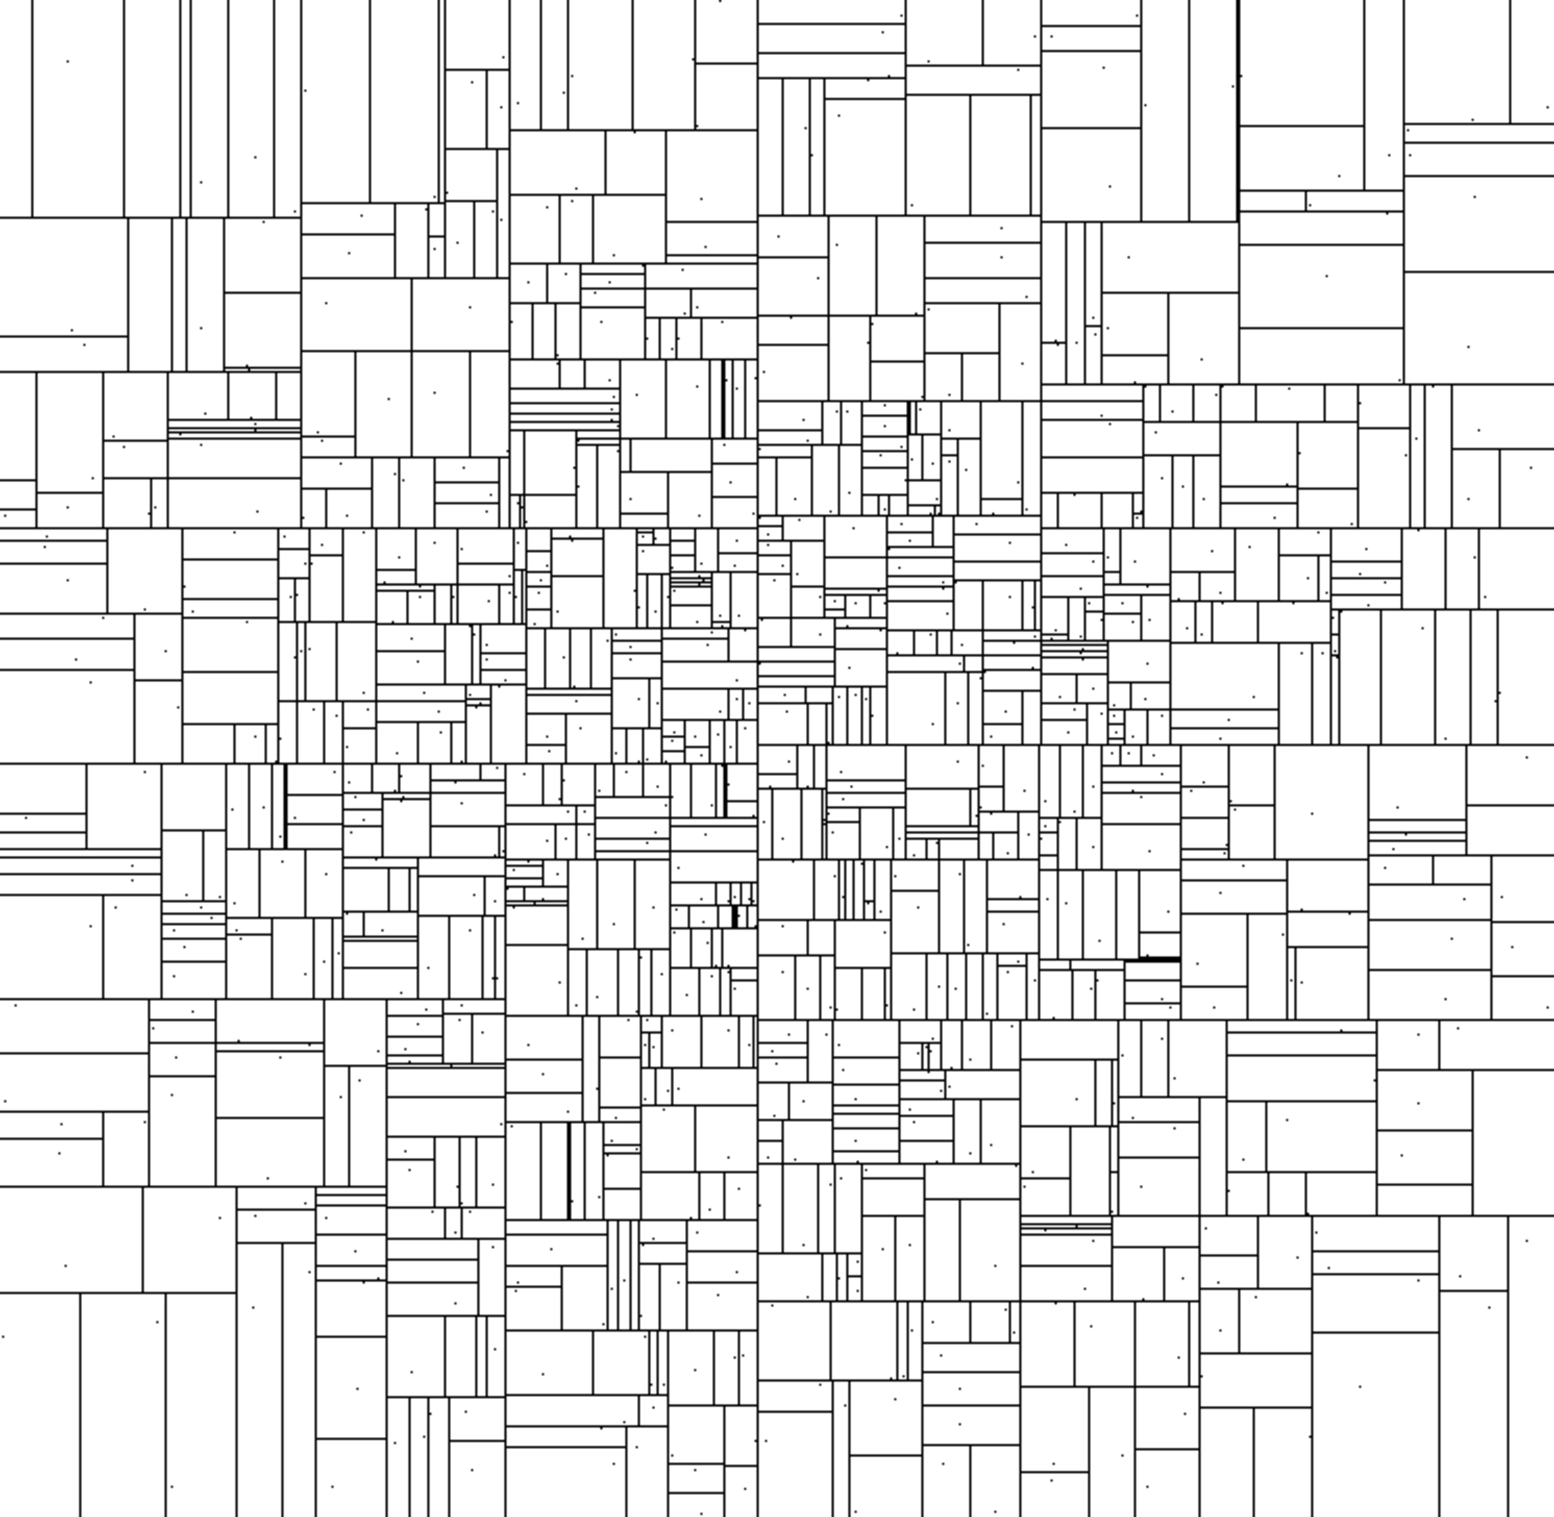
\includegraphics[width=0.8\columnwidth]{Figure1_kdtree}
  \end{center}
  \caption{\label{fig:kD-tree} The neighborhoods from a kD-tree
    constructed around a set of points that are normally distributed
    about the origin in two dimensions.  As the points become denser
    around the origin, the typical neighborhood gets smaller.  The
    interpolated PDF within a box of volume $V_i$ is $1/(N V_i)$,
    where $N$ is the total number of points (which is also the number
    of boxes).}
\end{figure}

In order to use the kD-tree interpolation as a jump proposal in an
MCMC, we must be able to quickly find the neighborhood associated with
a given point to compute the jump probability (see
Eq.~\ref{eq:p-accept}).  This can be accomplished in $\order{\log N}$
time and constant space with the following algorithm, which is a
standard binary tree search.  Given the point, $\vtheta_i$ and the
tree, $T$:
\begin{enumerate}
\item If $T$ contains exactly one sample point, then its box is the
  associated neighborhood.  Otherwise:
\item The tree $T$ has two sub-trees.  If the point $\vtheta_i$ is
  contained in the ``left'' sub-tree, then return to Step 1,
  considering this sub-tree; otherwise return to Step 1, considering
  the ``right'' sub-tree.
\end{enumerate}

\section{RJMCMC Efficiency}
\label{sec:efficiency}

In this section, we demonstrate the efficiency of the kD-interpolated
jump proposal on a toy model-comparison problem.  We draw $N = 100$
simulated data points from a $N(0,1)$ Gaussian distribution, and then
ask whether these data are better described by a model where they are
Gaussian distributed with unknown mean $\mu$ and standard deviation
$\sigma$
%
\be
p(x) = \frac{1}{\sqrt{2\pi} \sigma} \exp\left( - \frac{(x-\mu)^2}{2
    \sigma^2} \right)\ ,
\ee
%
or by a model where they are Cauchy distributed with mode $\alpha$
and width $\beta$
%
\be
p(x) = \frac{1}{\pi \beta \left( 1 + \left(\frac{x - \alpha}{\beta}\right)^2\right)}\ .
\ee
%
We take priors on $\mu$ and $\alpha$ to be uniform in $[-1,1]$, and
priors in $\sigma$ and $\beta$ to be uniform in $[0.5, 1.5]$.  With a
data set of 100 points, the relative uncertainty in determining the
parameters of the underlying distribution is approximately 10\%, so we
expect the posterior probabilities in the $(\mu,\sigma)$ and
$(\alpha,\beta)$ spaces to occupy only a few percent of the prior
volume.  The Cauchy distribution is much broader than the Gaussian (it
has no finite moments), so with \ilya{equal} model priors, the posterior
probability for the Gaussian model over the Cauchy model is extremely
large:
%
\be
\frac{p(\textnormal{Gaussian} | d)}{p(\textnormal{Cauchy}|d)} \sim 10^9.
\ee
%
In order to ensure that the RJMCMC produces samples in the Cauchy
model at all, we impose a model prior that favors the Cauchy model by
$5 \times 10^8$ relative to the Gaussian.  The evidence ratio between
the models for our chosen data set with these priors is
%
\be \frac{p(\textnormal{Gaussian} | d)}{p(\textnormal{Cauchy}|d)}
\equiv r = 1.15,
\ee
%
yielding a theoretical maximum acceptance rate of inter-model jumps of
$(1+1/r)/2 = 0.93$.

We obtain $10^4$ single-model MCMC samples by independently running
MCMC within each model, and use the kD-tree interpolation method
described above to propose inter-model jumps in an RJMCMC.  The
acceptance rate of inter-model jumps is approximately 0.8.  To explore
how the efficiency of the method degrades as the interpolation becomes
less accurate, we artificially truncated the kD tree with higher and
higher numbers of points in each box (this can be accomplished during
the neighborhood search phase by stopping the search for a box when
one is found containing the desired number of points).  For each
truncation choice, we performed an RJMCMC with the resulting
interpolated jump proposal.  The acceptance rate is plotted against
the number of single-model MCMC points per box (kD-tree leaf) in
Figure \ref{fig:acceptRate}.  The more points in each leaf of the tree
when the search is truncated, the lower the acceptance probability;
when points are drawn from the top level of the tree, the acceptance
probability asymptotes to the naive draw from the prior ($\sim 5\%$).

\begin{figure}
  \begin{center}
    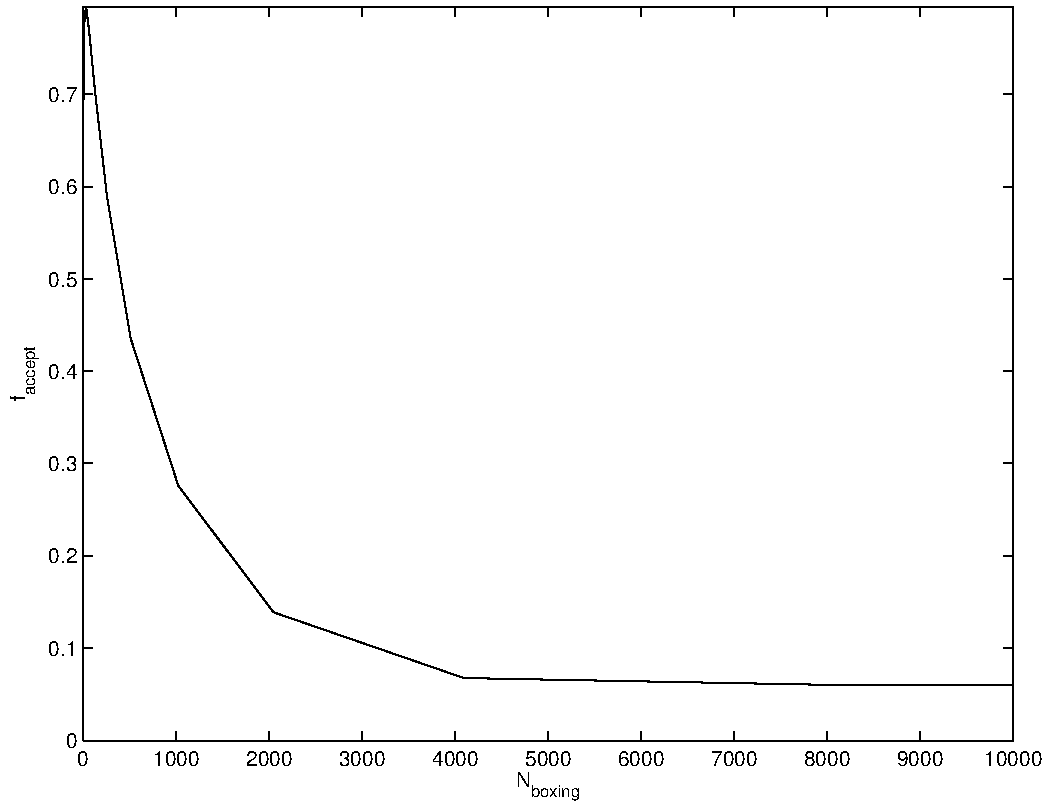
\includegraphics[width=0.8\columnwidth]{Figure2_acceptRate}
  \end{center}
  \caption{\label{fig:acceptRate} The inter-model \ilya{jump proposal} acceptance rate
    versus the number of points per box when the kD-tree neighborhood
    search is truncated.  As the number of points per box increases,
    and the interpolation becomes less accurate, the acceptance rate
    falls, asymptoting to the rate for naive draws from the uniform
    prior (about $5\%$ for this data set).}
\end{figure}

The relative error on the determination of the Bayes factor (evidence ratio) scales
with $1/\sqrt{N_{\textnormal{transitions}}}$, where
$N_{\textnormal{transitions}}$ is the number of inter-model
transitions in the RJMCMC.  Thus, as the acceptance rate of
inter-model jumps goes down, the RJMCMC must run longer to achieve a
desired accuracy in the evidence ratio.  By boosting the acceptance
rate of inter-model jumps, the interpolation method described above
can dramatically improve the runtime of an RJMCMC.

\section{kD-Interpolated Jump Proposal in Higher-Dimensional
  Single-Model MCMCs}
\label{sec:higherdim}

In the model selection example from Section \ref{sec:efficiency}, the
models have two-dimensional parameter spaces; in \cite{Farr2010} the
highest-dimensional model had five dimensions.  As the number of
dimensions increases the interpolation becomes more difficult for two
reasons.  First, the number of sample points required for a given
number of subdivisions in each dimension grows exponentially with
dimension \ilya{number}, so for reasonable numbers of points a high-dimensional kD
tree will have few subdivisions along each dimension.  Second, as
the dimensionality increases the volume ``at the \ilya{edges /} corners'' of each kD
tree box becomes more significant; this problem is even more
pronounced when the distribution of points does not align with the
coordinate axes along which the tree subdivides.  In this section, we
discuss practical solutions to this issue in the context of a
single-model MCMC, concluding with an example of a successful
application to gravitational-wave parameter estimation.

\ilya{[There is at least one paragraph missing here.  What's this "single-model MCMC" and why does it require PDF interpolation?  Are you running several MCMCs in succession as increasingly good approximations to the desired posterior?  Are you using higher-temperature chains to provide a jump proposal guess for lower temperatures?   More details needed.]}

To address the arbitrary orientation of points, \ilya{[Points don't have an orientation -- they are points!  Did you mean something like "To address significant covariance between samples"?]} 
 the modified jump
proposal does not descend to the leaf-nodes of the tree, but instead
stops descending whenever the number of points in the box falls below
a threshold, $\Nbox$. \ilya{[Is $\Nbox$ the threshold, or the actual number of points in the box -- it's defined to be the latter below \Eref{modforward}?]}  We then find the principal axes of the points
contained in this box and draw from a modified box which is aligned
with these axes and whose center is the mean of the points contained
within the rectangular box. \ilya{[Is the box drawn so that all $\Nbox$ samples fall inside it?  I think so, but it should be stated explicitly.]}  The new point \ilya{[The proposed jump?  Maybe this would be a good distinction between sample and point -- use point for proposed jumps and samples for the PDF samples being interpolated; if this was done consistently, this would be more clear...]} is chosen uniformly from
within the bounds of the modified box, subject to the restriction that
it also lie within the original, coordinate-aligned box.  Figure
\ref{fig:PCC} illustrates this two-box method.

\begin{figure}
  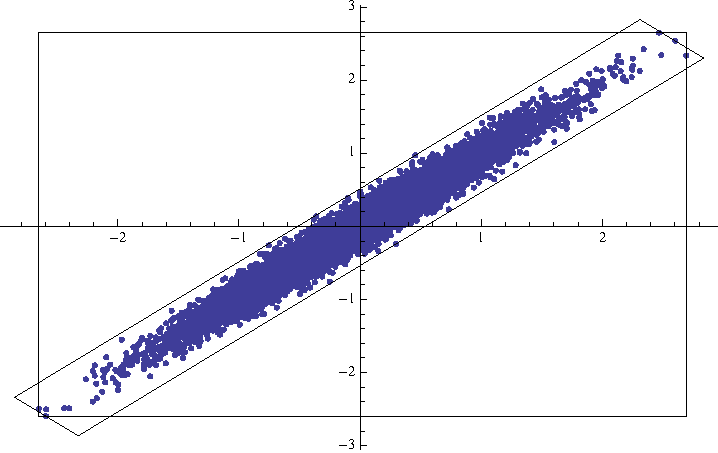
\includegraphics[width=0.8\columnwidth]{PCC}
  \caption{\label{fig:PCC} A two-dimensional illustration of the two
    boxes involved in the modified kD proposal.  The larger box
    aligned with the axes is the normal kD-tree box containing the
    given points, while the tighter box is the box from which the
    modified kd-interpolated jump proposal draws a point. }
\end{figure}

The forward jump probability for this jump proposal is given by
%
\bel{modforward} P(\vtheta_i \rightarrow \vtheta_{i+1}) =
\frac{\Nbox}{N \left(V \cap \Vbox \right)} , \ee
%
where N is the total number of points in the kD-tree, $\Nbox$ is the
number of points in the box containing $\vtheta_{i+1}$, $V$ is the
volume of the original box containing $\vtheta_{i+1}$ and $\Vbox$ is
the volume of the principal-component \ilya{[First time that "principal-component" is used to identify the diagonal sub-box...]} box containing $\vtheta_{i+1}$.

The backward jump probability is computed in a similar fashion by
finding the principal-component box that would contain the current set
of parameters: \ilya{[Probably not necessary -- we don't explicitly provide backward jump proposals in earlier sections]}
%
\bel{modbackward} P(\vtheta_{i+1} \rightarrow \vtheta_{i}) =
\frac{\Nbox'}{N\left(V' \cap \Vbox'\right)} , \ee
%
where $\Nbox'$ is the number of points in the original box containing
$\vtheta_i$, $V'$ is the volume of the kD box containing $\vtheta_i$,
and $\Vbox'$ is the volume of the principal-axes box containing
$\vtheta_i$.  Note, however, that the current parameters may lie in a
region of the kD box that does not intersect the principal axes box;
in this case, the backward jump probability is zero, and the algorithm
rejects the proposed step.  When used as the only jump proposal for an
RJMCMC, it is important that the kD tree proposal be capable of
proposing points in all allowed regions of parameter space; on the
other hand, when the kD proposal is used as one of several proposals
in the context of an MCMC, this is no longer a requirement.

It can also be advantageous, particularly in high-dimensional spaces,
to accumulate more points into the kD tree as the MCMC explores more
of the parameter space.  \ilya{[See above -- it's not clear what exactly we are doing here in general.]}
Because this introduces a dependence on the
previous states of the MCMC, the jump proposal is no longer
Markovian.  However, it remains \emph{asymptotically} Markovian \ilya{[And being asymptotically Markovian (whatever that actually means -- at least a reference?) -- is provably sufficient to guarantee that we sample from the equilibrium distribution even though we nominally violate detailed balance? (again, a reference?)]} , which
ensures that the equilibrium distribution of the MCMC is correct.  To
efficiently insert points into the tree as the chain accumulates them,
the algorithm from Section \ref{sec:kDTree} must be modified:
\begin{enumerate}
\item Instead of partitioning the point set at its median, we now
  partition the bounding box at its geometric center along a
  particular dimension, which cycles as we descend the tree levels.
  Note that this allows for empty boxes if all the points cluster to
  one side of the domain.
\item When inserting a point, we descend the tree to a leaf node,
  which now can be either empty or contain one point.  If it is empty,
  we insert the point at this node.  If it contains one point, we
  subdivide the appropriate dimension, and place both points into the
  two sub-boxes.  If both land in the same sub-box, we continue
  subdividing, until each box in the sub-sub-sub... tree contains one
  or zero points.
\end{enumerate}
Insertion of a point is $\order{\log N}$, since it involves a constant
amount of work per tree level, and there are $\log N$ tree levels.  \ilya{[No -- the number of tree levels can be arbitrarily large if the original samples are clustered into a very small region of the prior volume...]}
Neighborhood lookup proceeds as before, and is therefore also
$\order{\log N}$.  \ilya{[Perhaps $\order{\log N + \Nbox}$, since must recompile the inner bounding box every time -- and, depending on problem, $\Nbox$ could be $\gg \log N$?]}

We have implemented this modified kD tree proposal as one of many jump
proposals in the \texttt{LALInferenceMCMC} sampler
\cite{vanderSluys:2008a,Raymond:2010,Raymond2012}.
\texttt{LALInferenceMCMC} is a MCMC code \cite{lalinf_method}, based on the LIGO algorithms
library, designed to sample the posterior on parameters of \ilya{merging}
compact-object binaries (masses, orbital orientation, distance, sky
position, etc) \ilya{encoded in} their gravitational wave \ilya{signatures} in
Earth-based gravitational wave detectors like LIGO.  The simplest such
signal has a nine-dimensional parameter space, and the posterior often
includes near-degeneracies and multiple modes that make convergence of
the MCMC chain very slow with traditional proposals.  Figure
\ref{fig:accratio} shows the acceptance ratio for the kD-tree jump
proposal in such a simulation.  In spite of the very low acceptance
rate of the proposal, applying the kD-tree proposal to one out of
twenty proposed jumps improved the convergence time of the simulation
by a factor of two compared to the standard suite of proposals because
it is particularly efficient at producing ``mode-hopping'' jumps,
which are difficult to produce with the other proposals in
\texttt{LALInferenceMCMC}.  \ilya{[Again, what exactly is reported in this figure?  Results with a jump proposal based on an interpolated PDF (of what)?  A proposal that's being updated on the fly as more samples come in?]}

\begin{figure}
  \begin{center}
    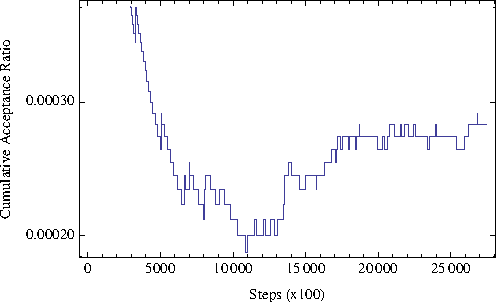
\includegraphics[width=0.8\columnwidth]{linearlog3}
  \end{center}
  \caption{\label{fig:accratio} The cumulative parameter acceptance
    ratio for the modified kD-interpolated jump proposal used in the
    \texttt{LALInferenceMCMC} code as a function of the number of
    steps (in hundreds). In spite of the small acceptance ratio, the
    kD tree proposal, applied to one in twenty proposed jumps,
    improved the convergence time of the sampler by a factor of two
    compared to using only the standard suite of proposals. \ilya{[I see structure in this figure (a high acceptance probability, followed by a dip, followed by an asymptote).  Is this a fluke, or do you always see this -- and, if so, why?  BTW, what's the autocorrelation length (just to give me a sense of scale, so I am not reading too much into meaningless fluctuations within an AC length)?]}}
\end{figure}

\section{Conclusion}
\label{sec:conclusion}

The need to compare evidences for multiple models arises in a large
variety of physical and astronomical contexts.  In this paper, we
described a technique that allows for efficient evidence
computations via a Reversible-Jump Markov chain Monte Carlo.  This
technique solves the usual problem of finding good inter-model jump
proposals in an RJMCMC by using a kD tree to quickly and accurately
interpolate an approximate posterior PDF from a single-model MCMC run,
and then proposing efficient inter-model
jumps \ilya{from} this interpolated PDF.

We demonstrated the efficiency of this technique on a toy
model-comparison problem described in Section \ref{sec:efficiency}.
We also successfully applied this technique to the problem of
selecting the best model for the observed distribution of black-hole
X-ray binary \ilya{masses}, as described in \cite{Farr2010}.  In addition to
model comparison, the PDF interpolation described here can be useful
in multi-step MCMCs to \sout{improve sampling efficiency by selecting
better jump proposal distributions} \ilya{propose jumps that can sample the parameter space more efficiently} or to test MCMC convergence. \ilya{[What are multi-step MCMCs (first mention)?  How do you use interpolation to test convergence?  I think it's bad form to introduce new ideas or new terminology in the penultimate paragraph of the paper with zero explanation.]}

We have made our implementation of the technique described in this
paper publicly available online at
\url{http://github.com/farr/mcmc-ocaml}, and also in the
\texttt{LALInferenceMCMC} sampler, at
\url{https://www.lsc-group.phys.uwm.edu/daswg/projects/lalsuite.html}.
We welcome readers to take advantage of this toolkit.


\section*{Acknowledgments}

We are grateful to Neil Cornish for interesting discussions.  IM
acknowledges support from the NSF Astronomy and Astrophysics
Postdoctoral Fellowship, award AST-0901985.  WF acknowledges support
from NSF grant AST0908930 and NASA grant NNX09AJ56G. DS acknowledges
support from a Northwestern University Summer Undergraduate Research Grant.  \ilya{This work has been partially supported by the UK Science and Technology Facilities Council.}

\section*{References}

\bibliography{paper}
%\bibliographystyle{unsrt}

\end{document}
